\section{Problem Description} %%%%%%%%%%%%%%%%%%%%%%%%%%%%%%%%%%%%%%%%%%%%%%%%%%
\label{sec:probl}

Pattern matching has been closely related to \emph{algebraic data types} and 
\emph{equational reasoning} since the early days of functional programming.
In languages like ML and Haskell an \emph{Algebraic Data Type} is a data type 
each of whose values is picked from a disjoint sum of (possibly recursive) data 
types, called \emph{variants}. Each of the variants is marked with a unique 
symbolic constant called \emph{constructor}. Constructors provide a convenient 
way of creating a value of its variant type as well as a way of discriminating 
its variant type from the algebraic data type through pattern matching.

C++ does not have direct support of algebraic data types, but they can usually 
be encoded with classes in a number of ways. One common such encoding is to 
introduce an abstract base class representing an algebraic data type with 
several derived classes representing variants. The variants can then be 
discriminated with either run-time type information (further referred to as 
\emph{polymorphic encoding}) or a dedicated member of a base class (further 
referred to as \emph{tagged encoding}). Object-oriented purists might argue that 
discrimination between the variants should be avoided at all costs through 
encapsulation. We disagree, however, as variants in traditional applications of 
algebraic data types are not implementation classes, but rather more-specialized 
interfaces.

By encoding algebraic data types with classes we alter their semantics in two 
important ways: we make them \emph{extensible} as new variants can be added by 
simply deriving from the base class, as well as \emph{hierarchical} as variants 
can be inherited from other variants and thus form a subtyping relation between 
themselves~\cite{Glew99}. This is not the case with traditional algebraic data 
types in functional languages, where the set of variants is \emph{closed}, while 
the variants are \emph{disjoint}. Some functional languages e.g. 
ML2000~\cite{ML2000} and Moby~\cite{Moby} were experimenting with 
\emph{hierarchical extensible sum types}, which are closer to object-oriented 
classes then algebraic data types are, but, interestingly, they did not provide 
pattern matching facilities on them. Working within a multi-paradigm  
programming language like C++, we will not be looking at algebraic data types in
the closed form they are present in functional languages, but rather in an 
open/extensible form discussed by Zenger~\cite{Zenger:2001}, Emir~\cite{EmirThesis}, 
L\"oh~\cite{LohHinze2006}, Glew~\cite{Glew99} and others. We will thus 
assume an object-oriented setting where new variants can be added later and form
subtyping relations between each other including those through multiple 
inheritance.

\subsection{Type Switch}

Consider a class \code{B} and a set of classes \code{Di} directly or indirectly 
inherited from it. An object is said to be of the \emph{most derived type} 
\code{D} if it was created by explicitly calling a constructor of that type.
The inheritance relation on classes induces a subtyping relation on them, which in 
turn allows objects of a derived class to be used in places where an object of a 
base class is expected. The type of variable or parameter referencing such an
object is called the \emph{static type} of the object. When object is passed by 
reference or by pointer, we might end up in a situation where the static type of an 
object is different from its most derived type, with the latter necessarily 
being a subtype of the former. The most derived class along with all its base classes 
that are not base classes of the static type are typically referred to as the 
\emph{dynamic types} of an object. At each program point the compiler knows the 
static type of an object, but not its dynamic types.

By \emph{type switch} we will refer to a programming language construct capable of 
uncovering a reference or a pointer to the dynamic type(s) of an object present in 
a given list of types.

Consider an object of (most derived) type \code{D}, pointed to by a variable of 
static type \code{B*}: e.g. \code{B* base = new D;}. A hypothetical type switch 
statement, not currently supported by C++, can look as following:

\begin{lstlisting}
switch (base)
{
case D1: s1;
 ...
case Dn: sn;
}
\end{lstlisting}

\noindent and can be given numerous plausible semantics:

\begin{itemize}
\setlength{\itemsep}{0pt}
\setlength{\parskip}{0pt}
\item \emph{First-fit} semantics will evaluate the first statement $s_i$ such 
      that $D_i$ is a base class of $D$
\item \emph{Best-fit} semantics will evaluate the statement corresponding to the 
      most derived base class $D_i$ of $D$ if it is unique (subject to 
      ambiguity)
\item \emph{The-only-fit} semantics will only evaluate statement $s_i$ if $D_i=D$.
\item \emph{All-fit} semantics will evaluate all statements $s_i$ whose guard 
      type $D_i$ is a subtype of $D$ (order of execution has to be defined)
\item \emph{Any-fit} semantics might choose non-deterministically one of the 
      statements enabled by all-fit
\end{itemize}

\noindent
The list is not exhaustive and depending on a language, any of these semantics 
or their combination might be a plausible choice. Functional languages, for 
example, often prefer first-fit, while object-oriented languages would typically 
be inclined to best-fit semantics. The-only-fit semantics is traditionally seen 
in procedural languages like C and Pascal to deal with discriminated union types. 
All-fit and any-fit semantics might be seen in languages based on predicate 
dispatching~\cite{ErnstKC98} or guarded commands~\cite{EWD:EWD472}, where a 
predicate can be seen as a characteristic function of a type, while logical 
implication can be seen as subtyping.

\subsection{Open and Efficient Type Switching}
\label{sec:poets}

The fact that algebraic data types in functional languages are closed allows for 
their efficient implementation. The traditional compilation scheme assigns unique 
tags to every variant of the algebraic data type and pattern matching is then 
simply implemented with a jump table over all tags. A number of issues in 
object-oriented languages makes this extremely efficient approach infeasible:

\begin{itemize}
\setlength{\itemsep}{0pt}
\setlength{\parskip}{0pt}
\item Extensibility
\item Subtyping
\item Multiple inheritance
\item Separate compilation
\item Dynamic linking 
\end{itemize}

\noindent
Unlike functional style algebraic data types, classes are \emph{extensible} 
whereby new variants can be arbitrarily added to the base class in the form of 
derived classes. Such extension can happen in a different translation unit or a
static library (subject to \emph{separate compilation}) or a dynamically linked 
module (subject to \emph{dynamic linking}). Separate compilation effectively 
implies that all the derived classes of a given class will only be known at link 
time, postponing thus any tag-allocation related decisions until then. The 
presence of dynamic linking effectively requires the compiler to assume that the
exact derived classes will only be known at run time, and not even at start-up 
time.

%and thus any tag allocation scheme should on one hand assume presence of 
%unknown tags and on the other -- the necessity of maintaing the same tags for 
%the commonly seen classes of each dynamic module.  

The \emph{subtyping} relation that comes along with extensibility through 
subclassing effectively gives every class multiple types -- its own and the 
types of all its base classes. In such a scenario it is natural to require that 
type switching can be done not only against the exact dynamic type of an object, 
but also against any of its base classes (subject to our substitutability 
requirement). This in itself is not a problem for functional-style tag 
allocation as long as the set of all derived classes is known, since the 
compiler can partition tags of all the derived classes according to chosen 
semantics based on classes mentioned in case clauses.
Unfortunately this will not work in the presence of dynamic linking as there 
might be new derived classes with tags not known at the time of partitioning and 
thus not mentioned in the generated jump table.

\emph{Multiple inheritance} complicates things further by making each class 
potentially belong to numerous unrelated hierarchies. Any tag allocation scheme 
capable of dealing with multiple inheritance will either have to assure that 
generated tags satisfy properties of each subhierarchy independently or use 
different tags for different subhierarchies. Multiple inheritance also 
introduces such a phenomenon as \emph{cross-casting}, whereby a user may request 
to cast pointers between unrelated classes, since they can potentially become 
base classes of a later defined class. From an implementation point of view this 
means that not only do we have to be able to check that a given object belongs 
to a given class (type testing), but also be able to find a correct offset to it 
from a given base class (type casting).

While looking at various schemes for implementing type switching we noted down a 
few questions that might help evaluate and compare solutions: 

\begin{enumerate}
\setlength{\itemsep}{0pt}
\setlength{\parskip}{0pt}
\item Can the solution handle base classes in case clauses?
\item Will it handle the presence of base and derived classes in the same match statement?
\item Will it work with derived classes coming from a DLL?
\item Can it cope with multiple inheritance (repeated, virtual)?
\item Can independently developed DLLs that either extend classes involved in 
      type switching or do type switching themselves be loaded together without 
      any integration efforts?
\item Are there any limitations on the number and or shape of class extensions?
\item What is the complexity of performing matching, based on the number of case clauses and 
      the number of possible types?
\end{enumerate}

The number of possible types in the last question refers to the number of subtypes 
of the static type of the subject, not all the types in the program. Several 
solutions discussed below depend on the number of case clauses in the match 
statement, which raises the question of how many such clauses a typical program 
might have. The C++ pretty-printer for Pivot we implemented using our pattern 
matching techniques originally had 8 match statements with 5, 7, 8, 10, 15, 17, 30 
and 63 case clauses each. While experimenting 
with probability distributions of various classes to minimize the number of 
conflicts (see \textsection\ref{sec:moc}), we had to associate probabilities 
with classes and implemented it with a match statement over all 160 nodes in the 
Pivot's class hierarchy. With Pivot having the smallest number of node kinds 
among the compiler frameworks we had a chance to work with, we expect a similar 
or larger number of case clauses in other compiler applications.

An obvious solution that will pass the above checklist can look like the following:

\begin{lstlisting}
if (D1* derived = dynamic_cast<D1*>(base)) { s1; } else
if (D2* derived = dynamic_cast<D2*>(base)) { s2; } else
...
if (Dn* derived = dynamic_cast<Dn*>(base)) { sn; }
\end{lstlisting}

\noindent
Despite the obvious simplicity, its main drawback is performance: a typical 
implementation of \code{dynamic_cast} might take time proportional to the 
distance between base and derived classes in the inheritance tree~\cite{XXXXX}.
What is worse, is that the time to uncover the type in the $i^{th}$ case clause 
is proportional to $i$, while failure to match will always take the longest. 
This linear increase can be seen in the Figure~\ref{fig:DCastVis1}, where 
the above cascading-if was applied to a flat hierarchy encoding an algebraic 
data type with 100 variants. The same type-switching functionality implemented 
with the visitor design pattern took only 28 cycles regardless of the case.
\footnote{Each case $i$ was timed multiple times to avoid fluctuations, turning 
the experiment into a repetitive benchmark described in 
\textsection\ref{sec:eval}. In a realistic setting the cost of double dispatch 
was varying between 52 and 55 cycles.}
This is more than 3 times faster than the 93 cycles it took to uncover even the 
first case with \code{dynamic_cast}, while it took 22760 cycles to uncover the 
last.

\begin{figure}[htbp]
  \centering
    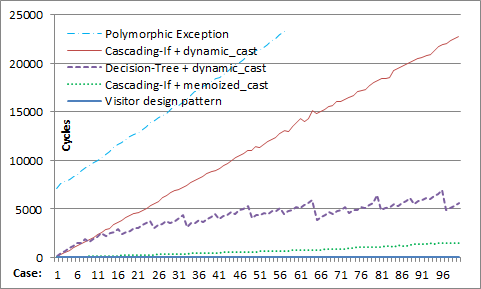
\includegraphics[width=0.47\textwidth]{DCast-vs-Visitors1.png}
  \caption{Type switching based on na\"ive techniques}
  \label{fig:DCastVis1}
\end{figure}

When the class hierarchy is not flat and has several levels, the above 
cascading-if can be replaced with a decision tree that tests base classes first 
and thus eliminates many of the derived classes from consideration. This 
approach is used by Emir to deal with type patterns in Scala~\cite[\textsection 
4.2]{EmirThesis}. The intent is to replace a sequence of 
independent dynamic casts between classes that are far from each other in the 
hierarchy with nested dynamic casts between classes that are close to each 
other. Another advantage is the possibility to fail early: if the type of the subject 
does not match any of the clauses, we will not have to try all the cases. 
A flat hierarchy, which will likely be formed by the leaves in even a multi-level 
hierarchy, will not be able to benefit from this optimization and 
will effectively degrade to the above cascading-if. Nevertheless, when 
applicable, the optimization can be very useful and its benefits can be seen in
Figure~\ref{fig:DCastVis1} under ``Decision-Tree + dynamic\_cast''. The class 
hierarchy for this timing experiment formed a perfect binary tree with 
classes number 2*N and 2*N+1 derived from a class with number N. The structure 
of the hierarchy also explains the repetitive pattern of timings.

The above solution either in a form of cascading-if or as a decision tree can be 
significantly improved by lowering the cost of a single \code{dynamic_cast}. 
We devise an asymptotically constant version of this operator that we call
\code{memoized_cast} in \textsection\ref{sec:memcast}. As can be seen from the graph 
titled ``Cascading-If + memoized\_cast'', it speeds up the above cascading-if 
solution by a factor of 18 on average, as well as outperforms the decision-tree 
based solution with dynamic\_cast for a number of case clauses way beyond those that can happen in 
a reasonable program. We leave the discussion of the technique until 
\textsection\ref{sec:memcast}, while we keep it in the chart to give perspective on 
an even faster solution to dynamic casting. The slowest implementation in the 
chart based on exception handling facilities of C++ is discussed in 
\textsection\ref{sec:xpm}.

The approach of Gibbs and Stroustrup~\cite{FastDynCast} employs divisibility of numbers to obtain a 
tag allocation scheme capable of performing type testing in constant time. 
Extended with a mechanism for storing offsets required for this-pointer 
adjustments, the technique can be used for extremely fast dynamic casting on 
quite large class hierarchies. The idea is to allocate tags 
for each class in such a way that tag of a class D is divisible by a tag of a 
class B if and only if class D is derived from class B. For comparison purposes 
we handcrafted this technique on the above flat and binary-tree hierarchies and 
then redid the timing experiments from Figure~\ref{fig:DCastVis1} using the fast 
dynamic cast. The results are presented in Figure~\ref{fig:DCastVis2}. For 
reference purposes we retained ``Visitor Design Pattern'' and ``Cascading-If + 
memoized\_cast'' timings from Figure~\ref{fig:DCastVis1} unchanged. Note that 
the Y-axis has been scaled-up 140 times, which is why the slope of 
``Cascading-If + memoized\_cast'' timings is so much steeper.

\begin{figure}[htbp]
  \centering
    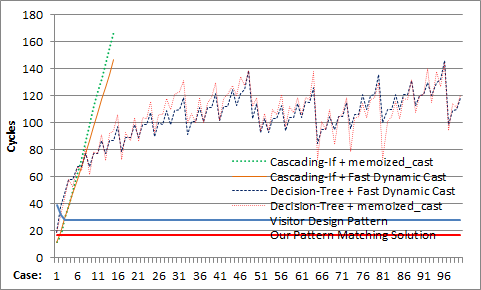
\includegraphics[width=0.47\textwidth]{DCast-vs-Visitors2.png}
  \caption{Type switching based on the fast dynamic cast of Gibbs and Stroustrup~\cite{FastDynCast}}
  \label{fig:DCastVis2}
\end{figure}

As can be seen from the figure the use of our memoized\_cast implementation can 
get close in terms of performance to the fast dynamic cast, especially 
when combined with decision trees. An important difference that cannot be seen 
from the chart, however, is that the performance of memoized\_cast is 
asymptotic, while the performance of fast dynamic cast is guaranteed. This 
happens because the implementation of memoized\_cast will incur an overhead of 
a regular dynamic\_cast call on every first call with a given most derived type. 
Once that class is memoized, the performance will remain as shown. Averaged over 
all calls with a given type we can only claim we are asymptotically as good as 
fast dynamic cast.

Unfortunately fast dynamic casting is not truly open to fully satisfy our 
checklist. The structure of tags required by the scheme limits the number of 
classes it can handle. A 32-bit integer is estimated to be able to represent 7 
levels of a class hierarchy that forms a binary tree (255 classes), 6 levels of 
a similar ternary tree hierarchy (1093 classes) or just one level of a hierarchy 
with 9 base classes -- multiple inheritance is the worst case scenario of the 
scheme that quickly drains its allocation possibilities. Besides, similarly to 
other tag allocation schemes, presence of class extensions in DLLs will likely 
require an integration effort to make sure different DLLs are not reusing prime 
numbers in a way that might result in an incorrect dynamic cast.

In view of the predictably-constant dispatching overhead of the visitor design pattern, 
it is clear that any open solution that will have a non-constant dispatching 
overhead will have a poor chance of being adopted. Multi-way switch on 
sequentially allocated tags~\cite{Spuler94} was one of the few techniques that 
could achieve constant overhead, and thus compete with and even outperform visitors. 
Unfortunately the scheme has problems of its own that make it unsuitable for 
truly open type-switching and here is why.

%To better understand the problem let us look at some existing solutions to type 
%switching that we found to be used in practice. 

%From our experience on this project we have noticed that we can only compete 
%with visitors when switch statements are implemented with a jump table. As soon 
%as compiler was putting even a single branch into the decision tree of cases, 
%the performance was degraded significantly. From this perspective we do not 
%regard solutions based on decision trees as efficient, since they do not let us 
%compete compete with the visitors solution.

The simple scheme of assigning a unique tag per variant (instantiatable class 
here) will not pass our first question because the tags of base and derived 
classes will have to be different if the base class can be instantiated on its 
own. In other words we will not be able to land on a case label of a base class, while 
having a derived tag only. The already mentioned partitioning of tags of derived 
classes based on the classes in case clauses also will not help as it assumes 
knowledge of all the classes and thus fails extensibility through DLLs.

In practical implementations hand crafted for a specific class hierarchy, tags 
often are not chosen arbitrarily, but to reflect the subtyping relation of the 
underlain hierarchy. Switching on base classes in such a setting will typically 
involve a call to some function $f$ that converts derived class' tag into a base 
class' tag. An example of such a scheme would be having a certain bit in the tag 
set for all the classes derived from a given base class. Unfortunately this 
solution creates more problems than it solves.

First of all the solution will not be able to recognize an exceptional case 
where most of the derived classes should be handled as a base class, while a few 
should be handled specifically. Applying the function $f$ puts several different 
types into an equivalence class with their base type, making them 
indistinguishable from each other.

Secondly, the assumed structure of tags is likely to make the set of tags 
sparse, effectively forcing the compiler to use a decision tree instead of a jump 
table to implement the switch. Even though conditional jump is reported to be 
faster than indirect jump on many computer architectures~\cite[\textsection 
4]{garrigue-98}, this did not seem to be the case in our experiments. Splitting 
of a jump table into two with a condition, that was sometimes happening because 
of our case label allocation scheme, was resulting in a noticeable degradation of 
performance in comparison to a single jump table.

Besides, as was seen in the scheme of Gibbs and Stroustrup, the assumed 
structure of tags can also significantly decrease the number of classes a given 
allocation scheme can handle. It is also interesting to note that even though 
their scheme can be easily adopted for type switching with decision trees, it is 
not easily adoptable for type switching with jump tables: in order to obtain 
tags of base classes we will have to decompose the derived tag into primes and 
then find all the dividers of the tag present in case clauses.

To summarize, truly open and efficient type switching seems to be a non-trivial 
problem. The implementations we found in the literature were either open or 
efficient, but not both. Efficient implementation was typically achieved by 
sealing the class hierarchy and using a jump table. Without sealing, the implementation 
was resorting to decision trees and type testing, which was not efficient.
We are unaware of any efficient tag allocation scheme that can be used in a 
truly open scenario.
